\documentclass[10pt]{beamer}

%STANDARD PREAMBLE
%https://tex.stackexchange.com/questions/68821/is-it-possible-to-create-a-latex-preamble-header
%\usepackage{/Users/mwojno01/Repos/latex_preamble/beamer_preamble}
\usepackage{/Users/miw267/Repos/csci246_spring2025/slides/preambles/beamer_preamble_for_CSCI246}


%%%
% SPECIFIC TO THIS DOCUMENT 
%%%
\let\warning\relax
\usepackage{fourier} % has warning  and danger symbols. However, it makes the bottoms tuff bold. 

\renewcommand{\ELBO}{\texttt{ELBO}}
\renewcommand{\Q}{\mathcal{Q}}


%%%%
% DOCUMENT 
%%%
\title{03/10/2026: Variational Inference}
\author{Reference: \textit{Variational Inference: An review for statisticians}}
\date{CSCI 546: Diffusion Models}

\begin{document}
\maketitle

\begin{frame}{Table of contents}
  \setbeamertemplate{section in toc}[sections numbered]
  \tableofcontents[hideallsubsections]
\end{frame}


\section{Course Logistics}


\begin{frame}
\begin{center}

\includegraphics[width=.6\textwidth]{images/DataFest 2026 blue.pdf}	
\end{center}
\end{frame}



\begin{frame}
\begin{myredbox}[title=Lightning Chats]
\begin{itemize}
	\item After Spring Break, any class meeting associated with a reading will have one $\approx$ 10 minute peer \textbf{lightning chat}. \pause 
	\item The lightning chats will be given in groups of two. I will do the best I can to assign groups based on your preferences. \pause 
	\item By Thursday, please bring in a list of three readings that are particular interest to you.  You can order them if you want.  You can name people you'd like to work with. 
\end{itemize}
\end{myredbox}
\end{frame}


\begin{frame}{Reading Survey}

\begin{enumerate}
	\item What is variational inference? Why is it useful?
	\item Choose one of the following, and describe what it is:  evidence lower bound, mean field. 
\end{enumerate}
	
\end{frame}



\section{Good, Bad, Ugly, Beautiful}

\begin{frame}[standout]
Good, Bad, Ugly, Beautiful
\end{frame}

\section{Overview of Variational Inference}



%%%%%%%%%%%%%%%%%%%%%%%%%%%%%%%%%%%%%%%%%%%%%%%%%%


\begin{frame}{Statistical inference in Bayesian models}
\footnotesize


\metroset{block=fill}
\begin{block}{Bayes' rule for densities}


\[ \underset{posterior}{p(\+u|\+x)} = \df{ \underset{likelihood}{p(\+x|\+u)} \quad  \underset{prior}{p(\+u)} }{ \underset{evidence}{p(\+x)}} \] %= \dfrac{p(\+x | \+u) p(\+u)}{\int p(\+x | 
%\+u) p(\+u)  \wrt{\+u}}  \]

where 
\begin{itemize}
\item $\+x$: observed data 
\item $\+u$: unobserved random variables
\end{itemize}
\end{block}

\pause 
\vfill 
\metroset{block=fill}
\begin{block}{A potential barrier to inference}

\begin{minipage}{0.6\textwidth}
By Bayes' rule, we cannot get the posterior without the \textbf{evidence}
%
\begin{align*}
p(\+x) & \overset{\text{\red{\danger}}}{=}  
\ds\int p(\+x, \+u)  \wrt{\+u}
\end{align*}
%
\end{minipage}
\hfill
\begin{minipage}{0.38\textwidth}
\centering

\includegraphics[width=.7\textwidth]{images/danger.png}
\end{minipage}
%
\pause 
\vfill 
Often this integral is \alert{intractable.}
\end{block}

	
\end{frame}


\begin{frame}{Approximate Bayesian Inference}

The two most prominent strategies for handling intractable posteriors are \textbf{Markov Chain Monte Carlo (MCMC)} and \textbf{Variational Inference (VI)}.  \pause 
\begin{itemize}
\item \textit{MCMC}  uses \alert{sampling}.  We construct a Markov chain over model parameters.  The stationary distribution is the posterior.  We approximate the posterior with samples. \pause 
\item \textit{VI} uses \alert{optimization}.  A tractable approximating family is chosen, and parameters are optimized to be close to the posterior.
\end{itemize}

\end{frame}

\begin{frame}{Variational Inference vs MCMC}

Variational Inference scales better to large datasets.

\begin{figure}
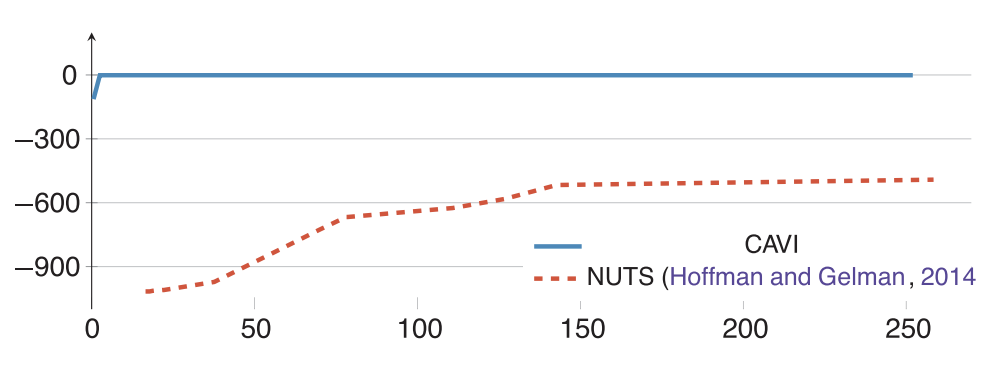
\includegraphics[width=\textwidth]{images/CAVI_vs_HamiltonianMCMC}
\caption{ Comparison of Coordinate Ascent Variational Inference (CAVI) to a Hamiltonian Monte Carlo-based sampling technique.  The plot shows log predictive likelihood on a test set by training time (minutes).  CAVI fits a Gaussian mixture model to 10,000 images in less than a minute.}
\end{figure}
\vfill
\tiny Blei, D. M., Kucukelbir, A., \& McAuliffe, J. D. (2017). Variational inference: A review for statisticians. Journal of the American statistical Association, 112(518), 859-877.
\end{frame}



%%%%%%%%%%%%%%%%%%%%%%%%%%%%%%%%%%%%%%%%%%%%%%%%%%

\begin{frame}{Variational Inference: An Illustration}

 \begin{minipage}[t][.9\textheight]{\textwidth}
  
Here we approximate an probability density by finding the best approximation from tractable family $\Q = \{ \text{10-component Gaussian mixture models} \}$ 

\begin{columns}[t]
\column{.5\textwidth}
\centering
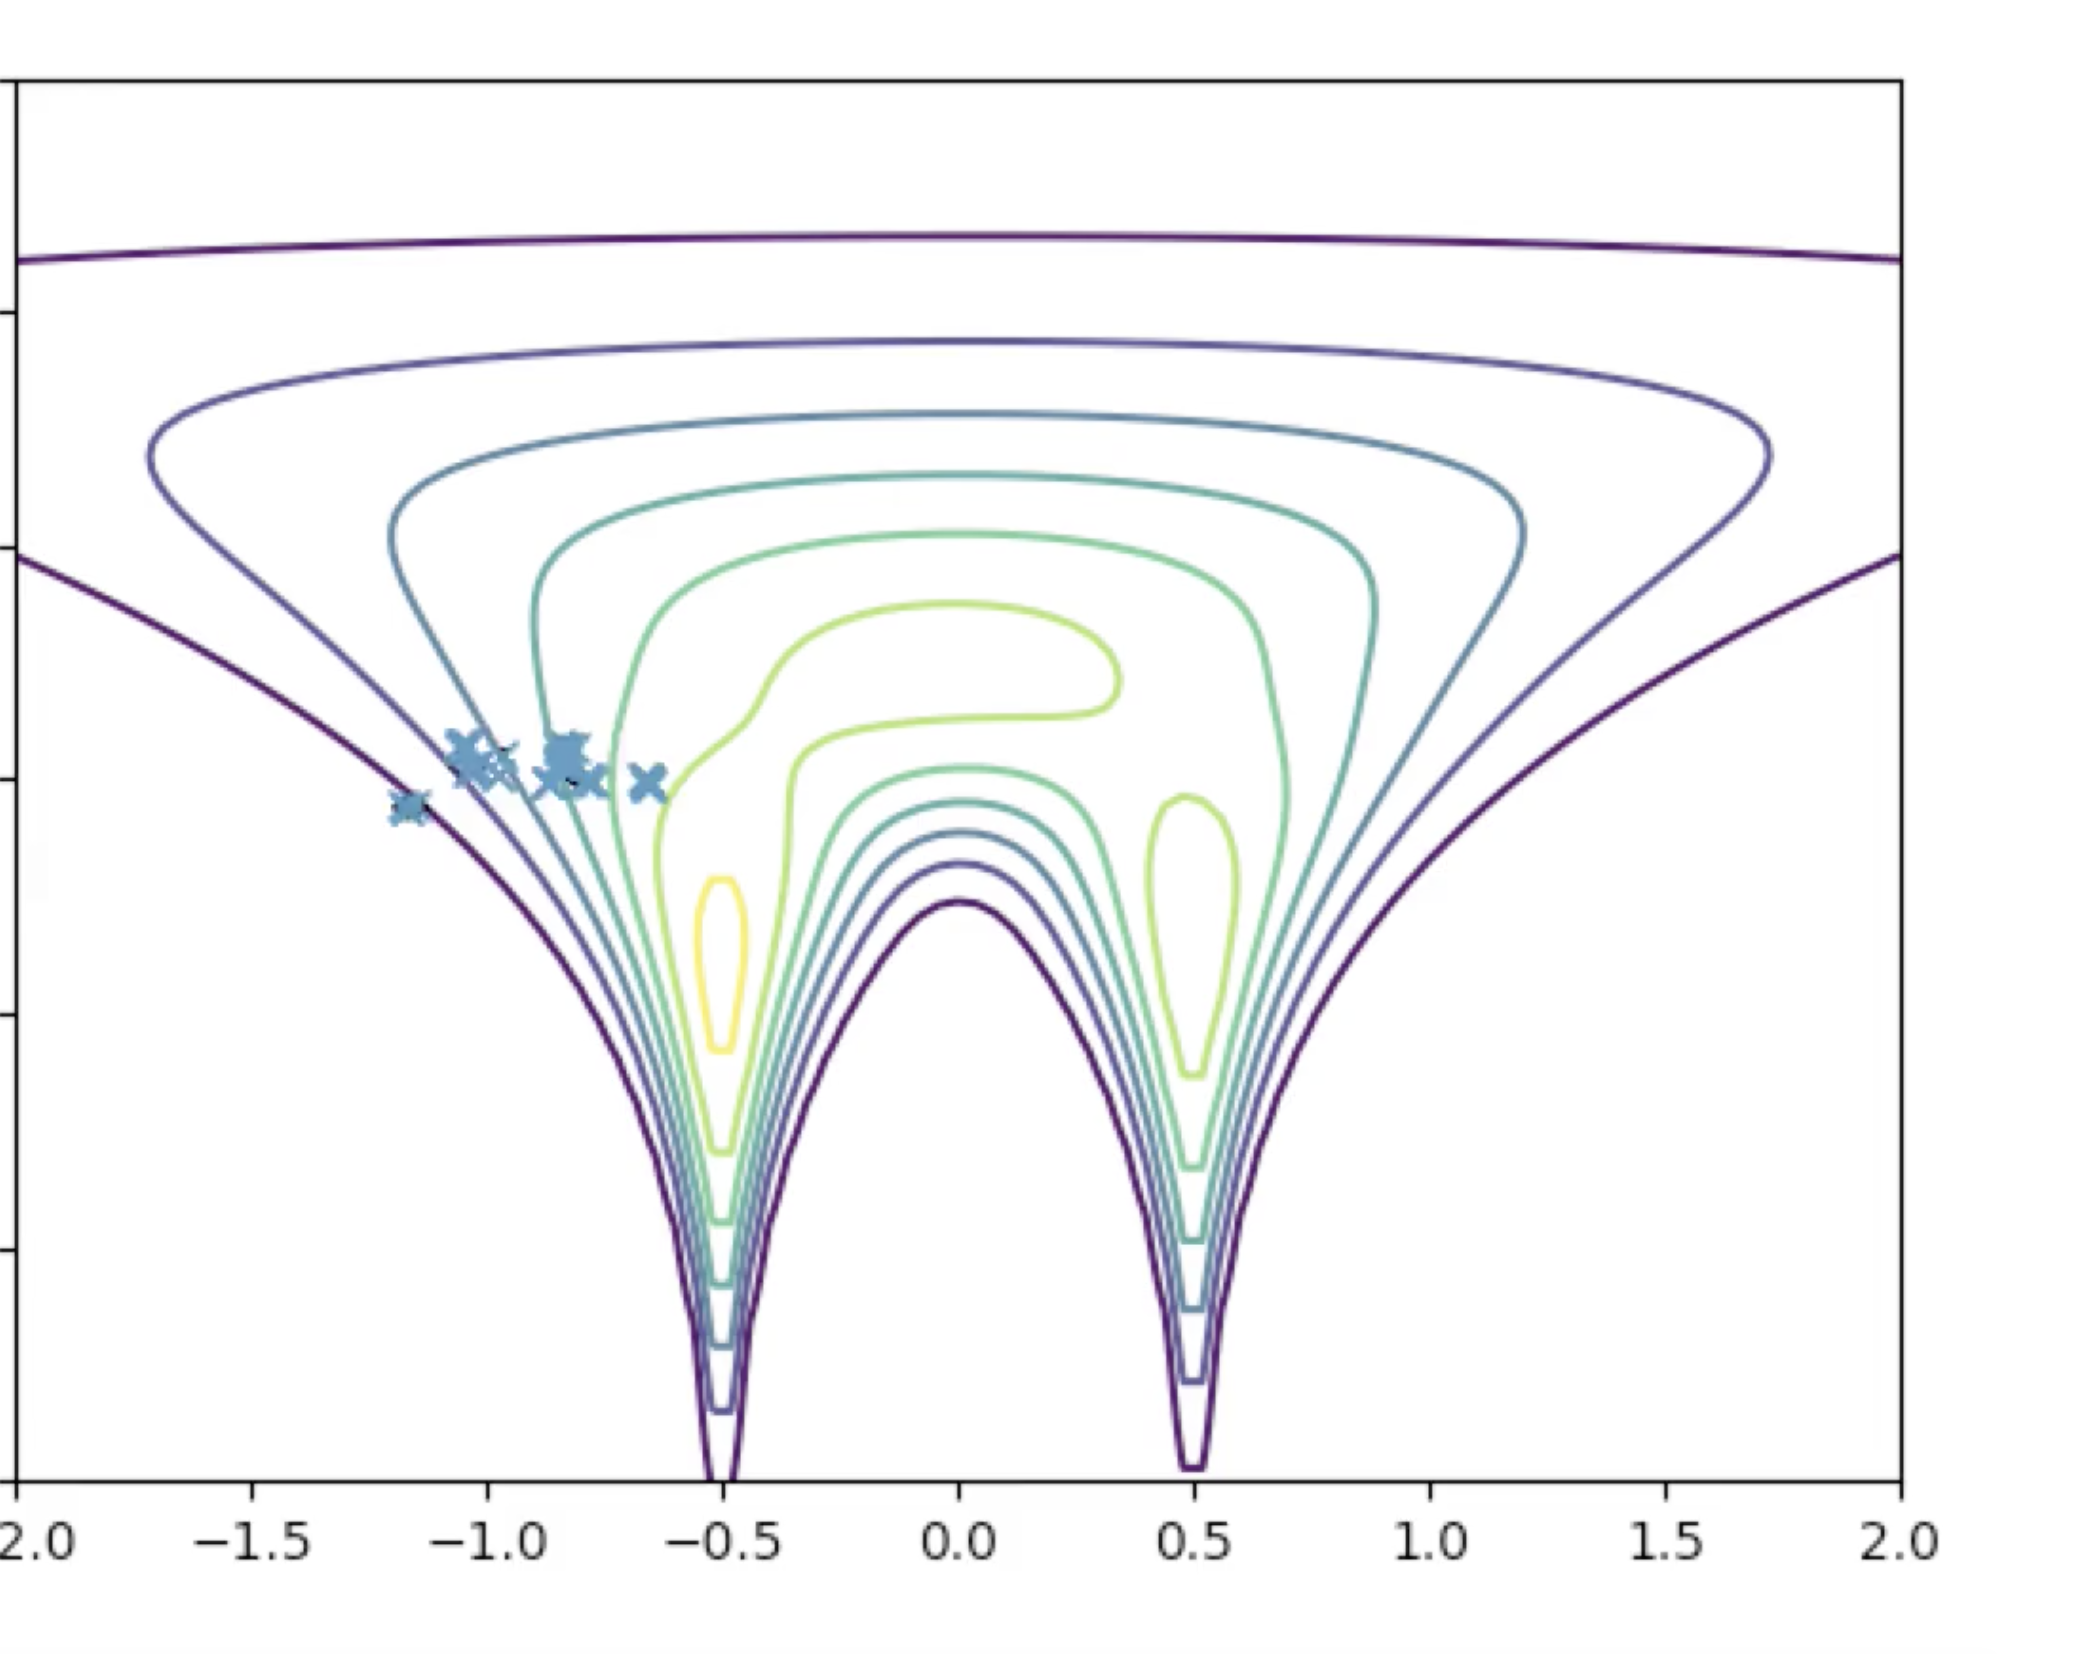
\includegraphics[width=.7\textwidth]{images/intro_animation_1.png}\\
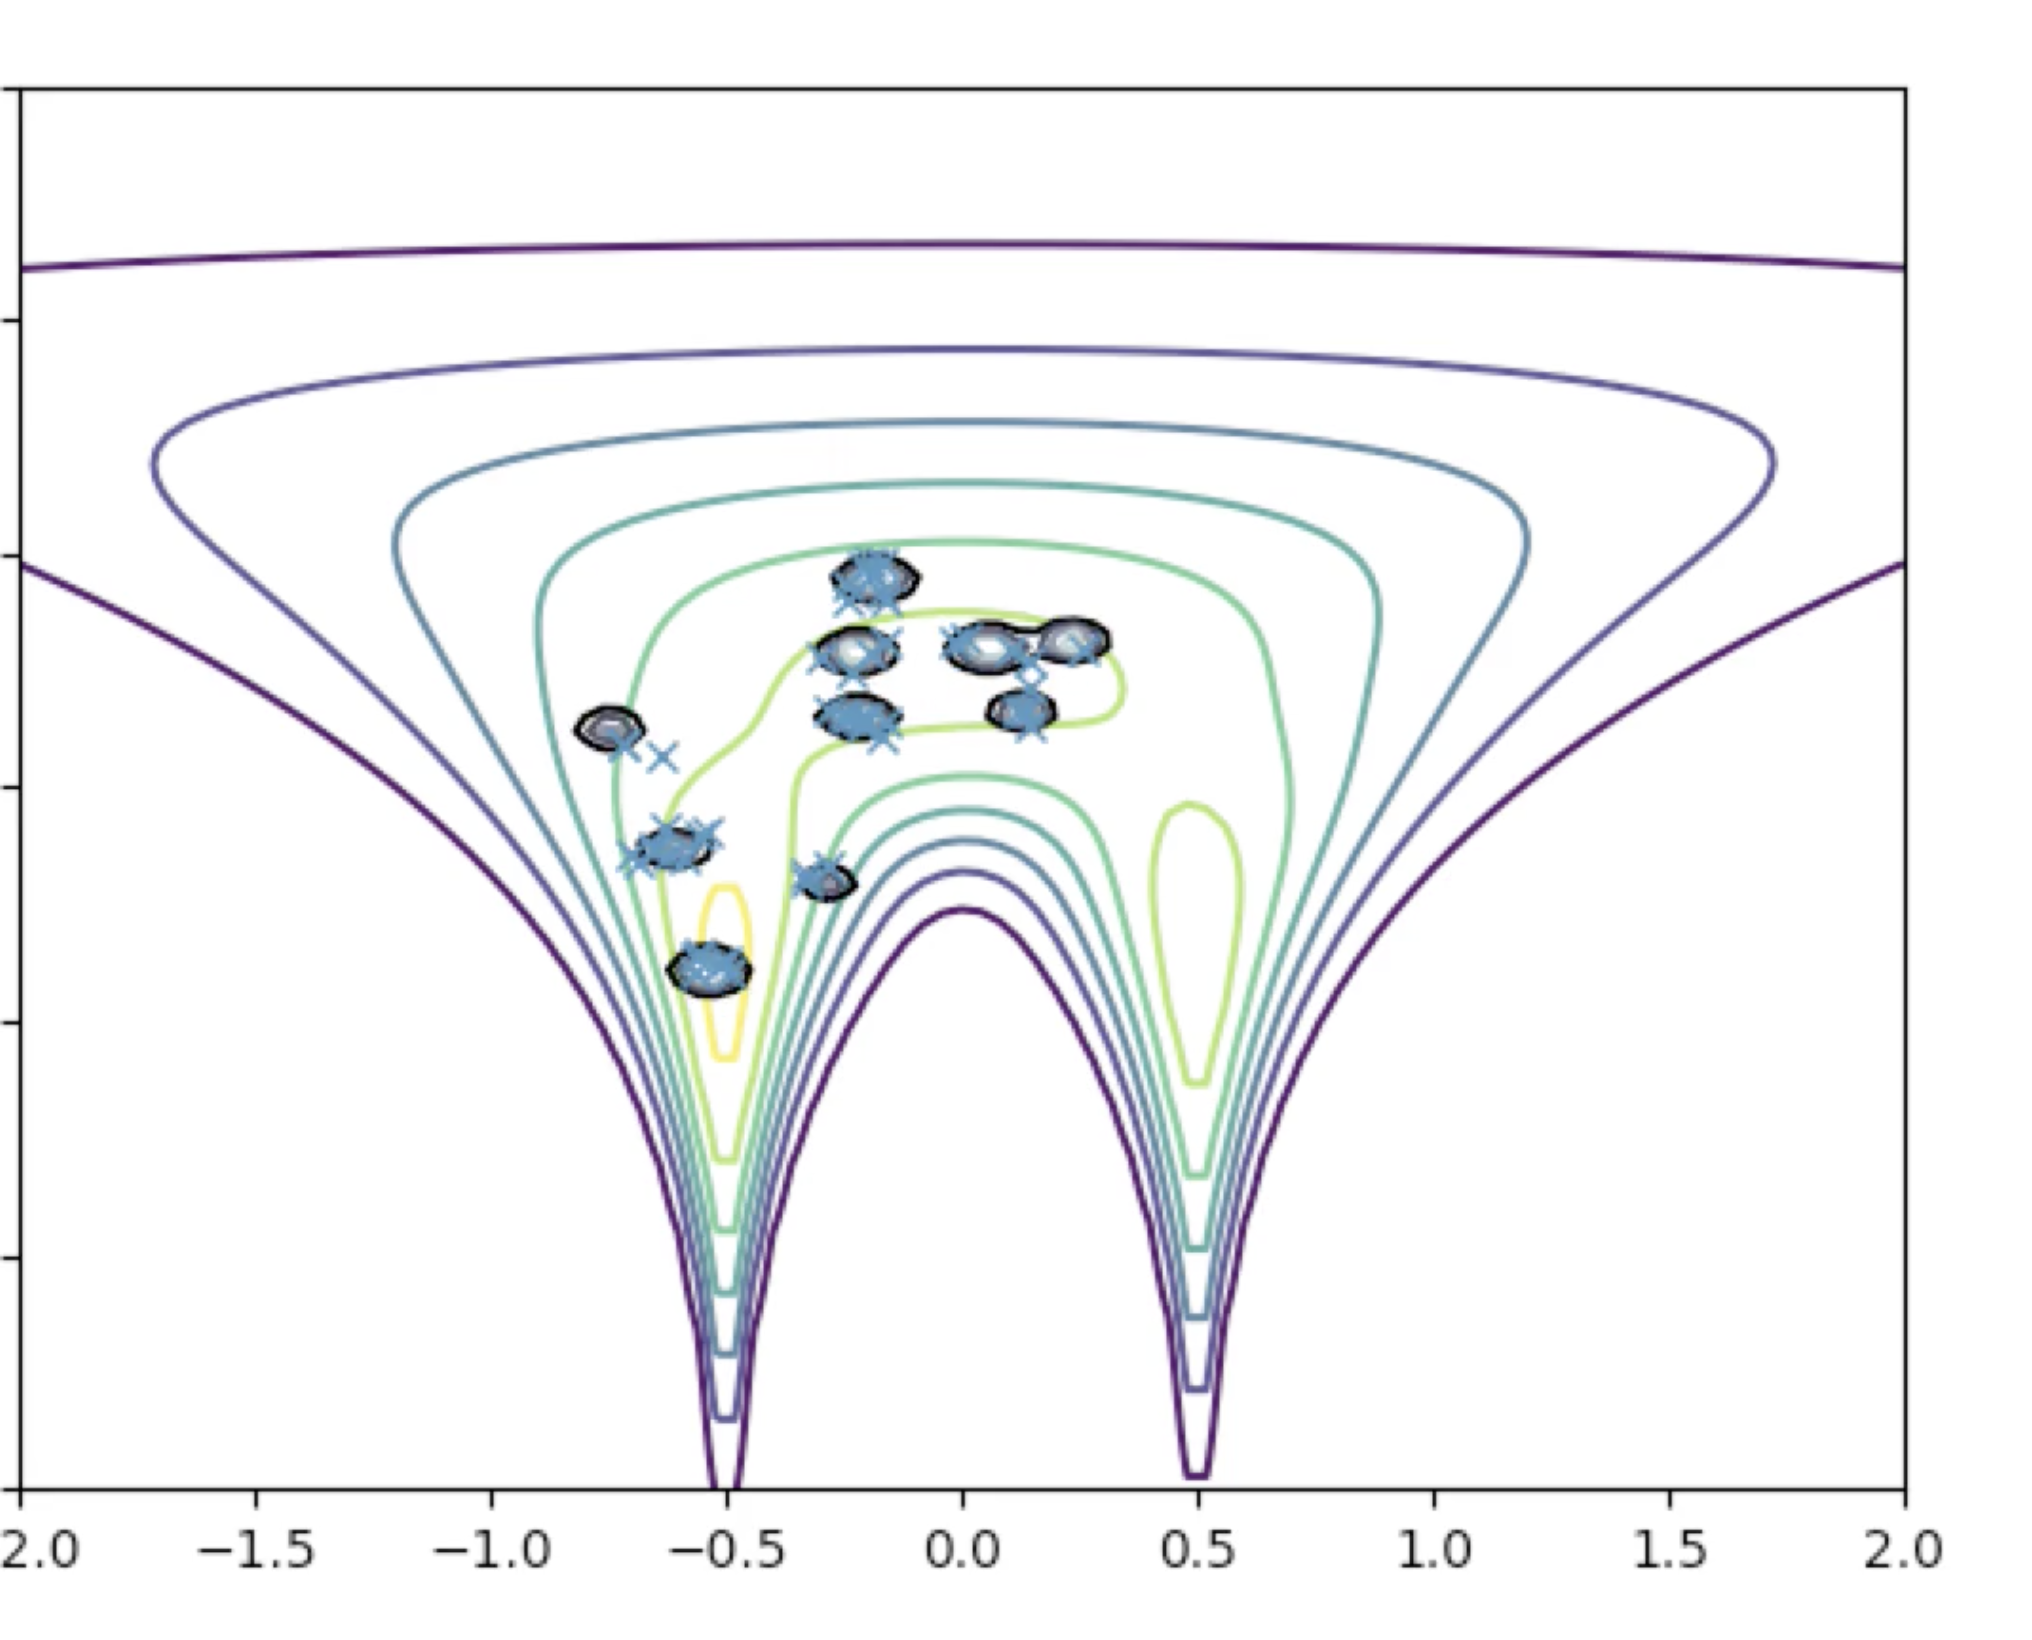
\includegraphics[width=.7\textwidth]{images/intro_animation_2.png}
\column{.5\textwidth}
\centering
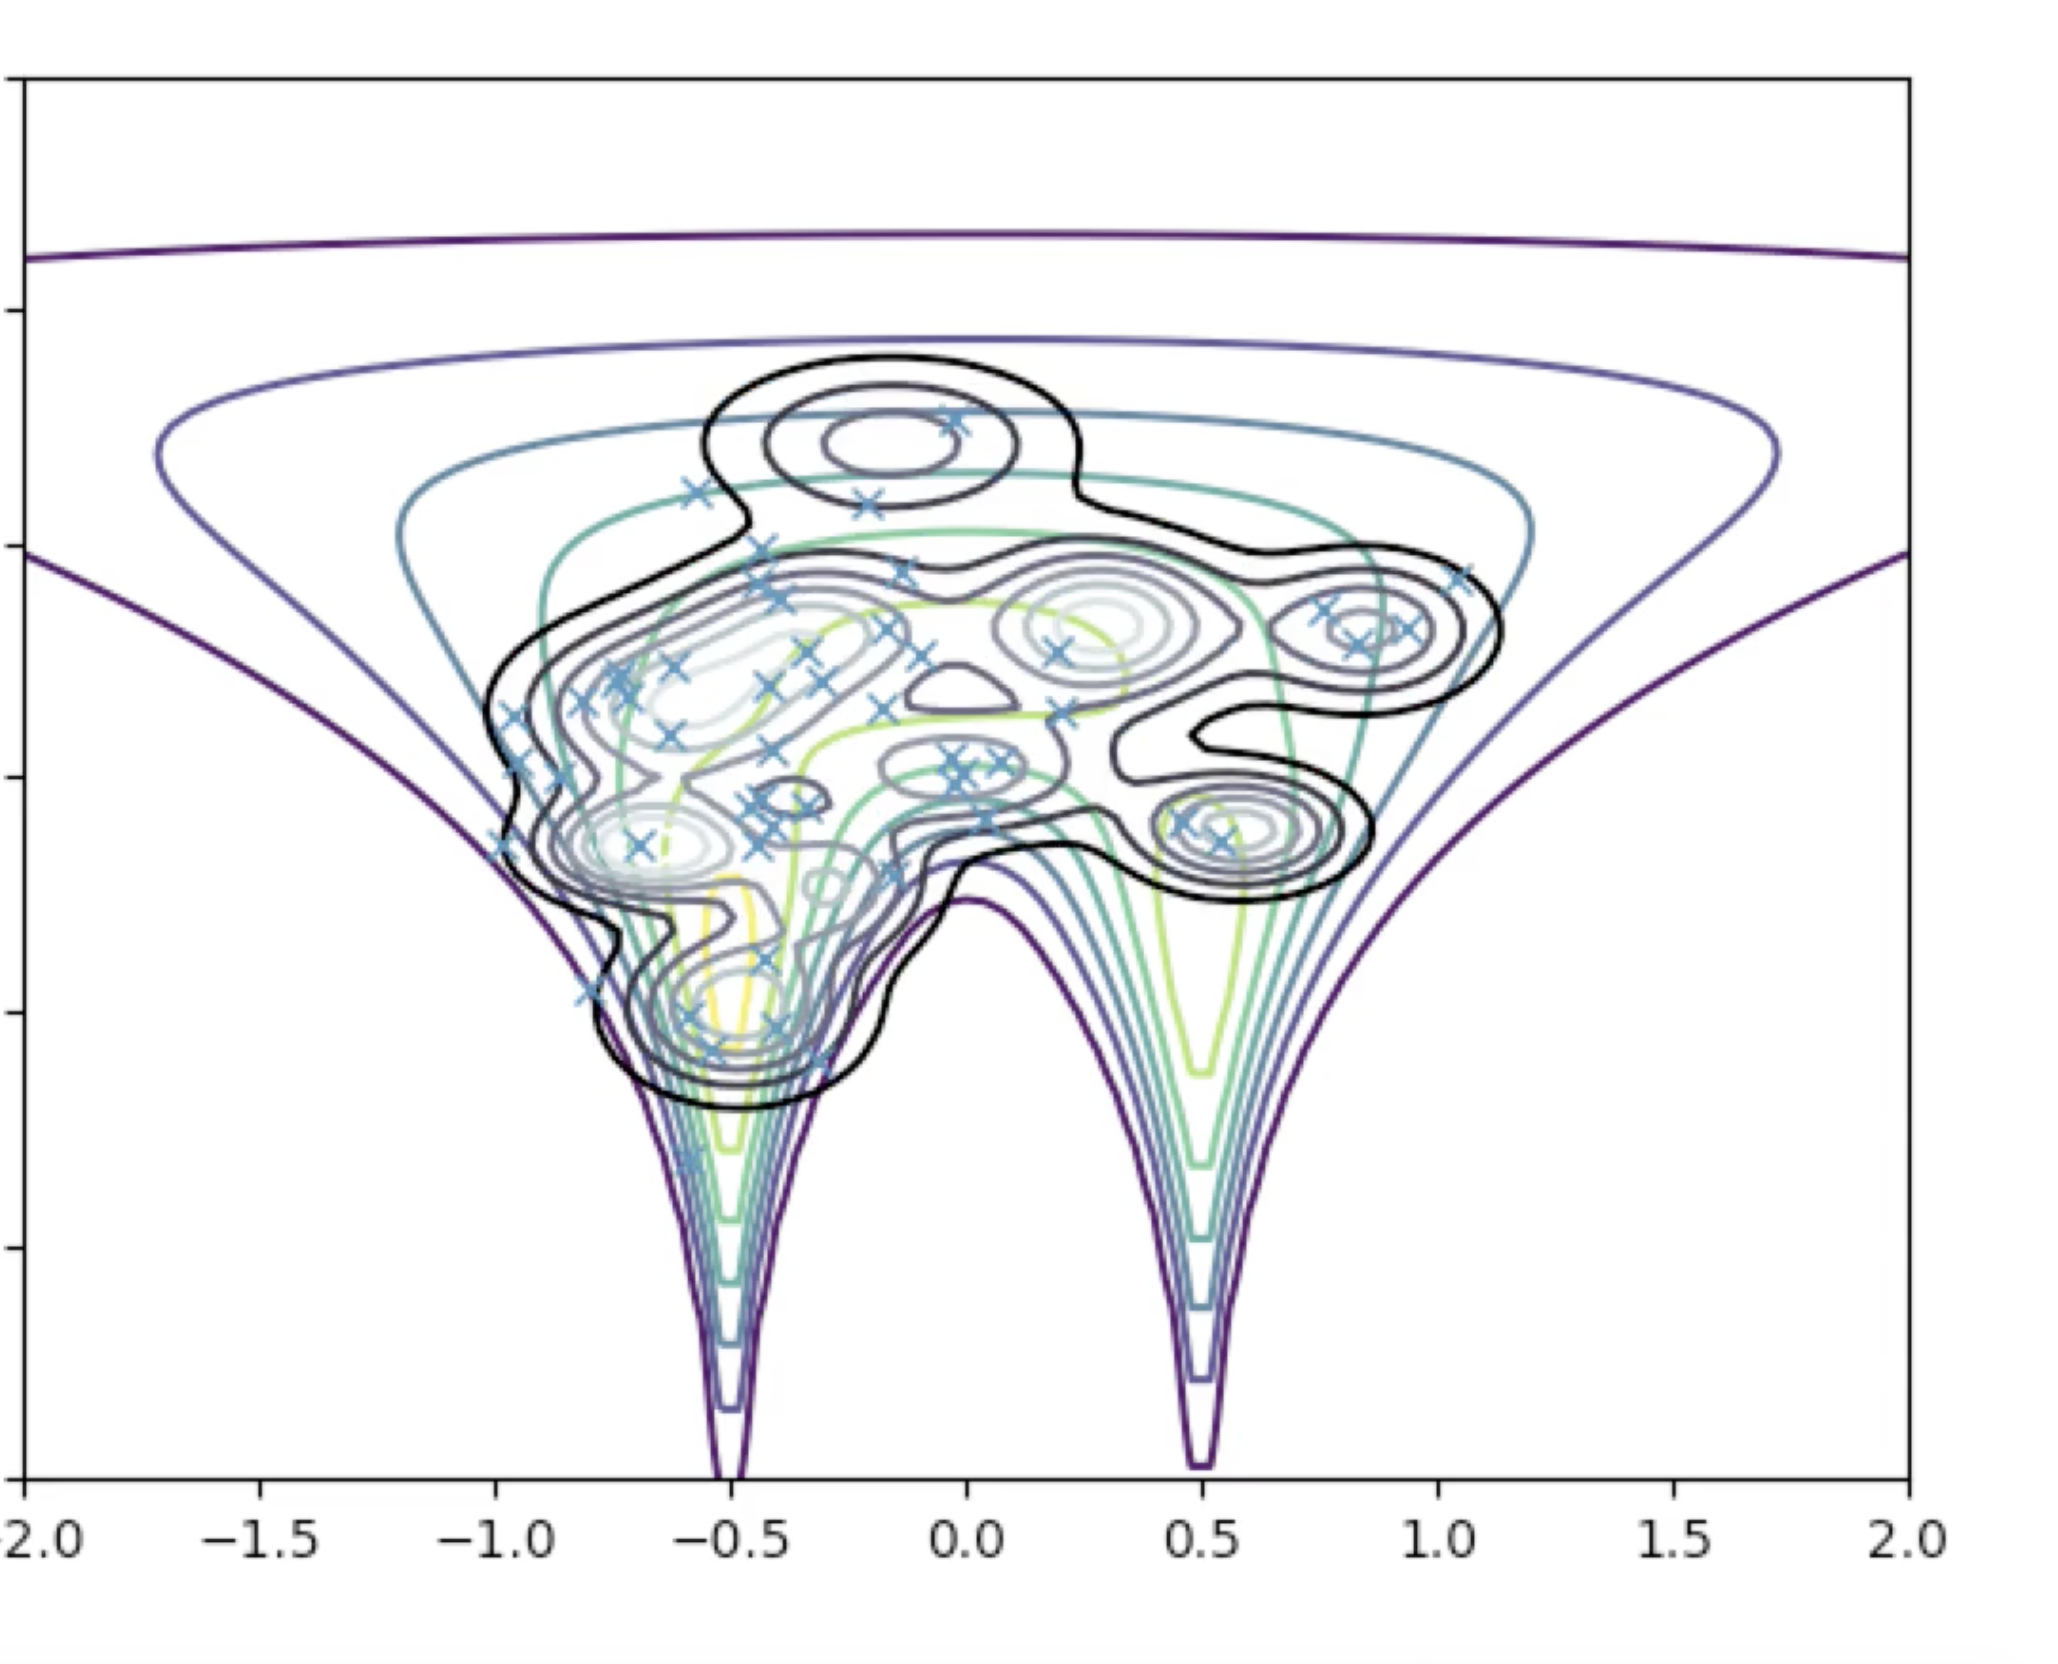
\includegraphics[width=.7\textwidth]{images/intro_animation_3.png}\\
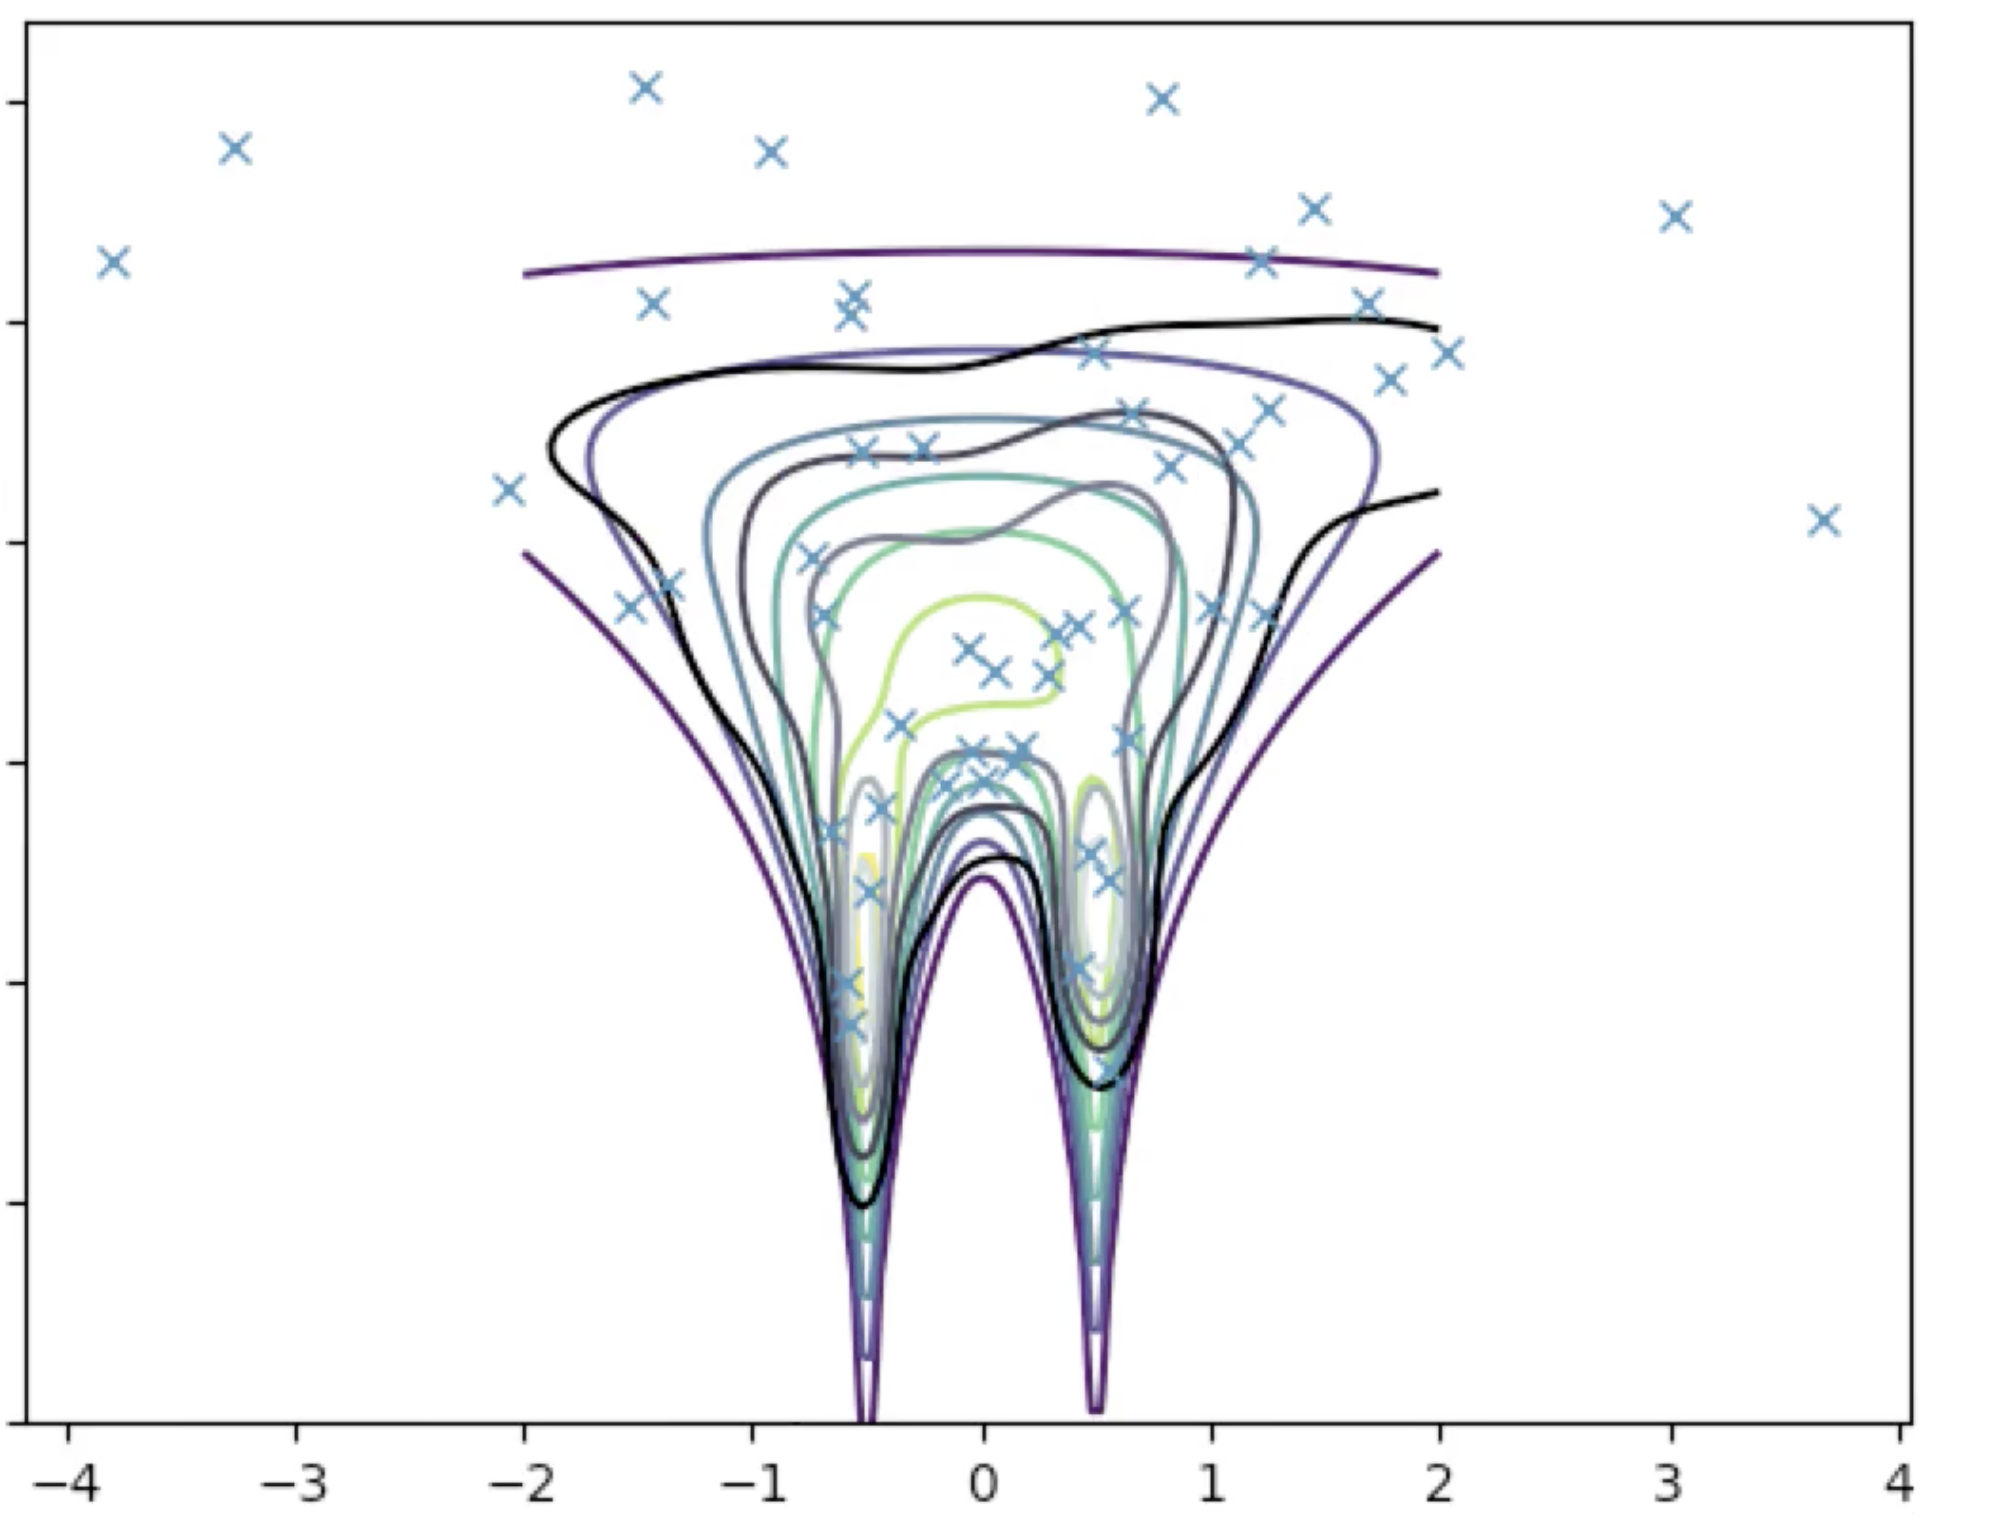
\includegraphics[width=.7\textwidth]{images/intro_animation_4.png}
\end{columns}

\vfill

%\tiny Ranganath, R., Gerrish, S., \& Blei, D. (2014, April). Black box variational inference. In Artificial Intelligence and Statistics (pp. 814-822).
  \end{minipage}
  
\end{frame}

%%%%%%%%%%%%%%%%%%%%%%%%%%%%%%%%%%%%%%%%%%%%%%%%%%
\begin{frame}{How variational inference works}
 

We construct a lower bound on the {\small (log)} evidence. 

\vfill 
\only<2->{
\metroset{block=fill}
\begin{block}{Evidence Lower Bound (ELBO)}
Let $\blue{q}$ be any probability density over $\+u$. Then:

\begin{align*}
\only<2->{\ln p(\+x) & = \ln \ds\int  p(\+u, \+x) \wrt{\+u}}  \\ 
\only<3->{& = \ln \ds\int  \blue{q(\+u)} \; \df{p(\+u, \+x  )}{\blue{q(\+u)}} \wrt{\+u}}  \\ 
\only<4->{& \stackrel{Jensen's}{\geq} \ds\int  q(\+u) \; \ln \bigg( \df{p(\+u, \+x)}{q(\+u)} \bigg) \wrt{\+u}} \\
\only<4->{& : = \ELBO(q)} 
\end{align*}
\end{block} 
}

\only<5->{We want to find $q \in \mathcal{Q}$ to maximize the $\ELBO$.}
 

\end{frame} 



%%%%%%%%%%%%%%%%%%%%%%%%%%%%%%%%%%%%%%%%%%%%%%%%%%%
\begin{frame}{Maximizing the $\ELBO$ \\ is minimizing the KL divergence to the posterior}  

%The variational density $q \in \mathcal{Q}$  which maximizes the \VLBO also minimizes the KL divergence from the target posterior $p(\+u \cond \+x, \+c)$ %to the variational density. 

By definition, the \texttt{KL} divergence from the target posterior to the variational density is given by
\begin{equation*}
\texttt{KL} (q(\+u) \parallel p(\+u \cond \+x)) =  \E_q \bigg[\log \df{q(\+u )}{p(\+u \cond \+x)} \bigg] 
\end{equation*}

\pause 
\vfill 
 

%\begin{equation*}
% \texttt{KL} (q(\+u) \; || \; p(\+u \cond \+x, \+c)) =  \E_q[\log q(\+u )]  - \E_q[ \log p(\+u \cond \+x, \+c)] 
%\end{equation*}

By the chain rule, we get 
\begin{align*} 
 \texttt{KL} (q(\+u) \parallel p(\+u \cond \+x)) & =  \explaintermbrace{$-\ELBO(q)$}{\E_q[\log q(\+u )]  - \E_q[ \log p(\+u, \+x)]} &&+ \explaintermbrace{constant}{\log p(\+x)} \\
 \end{align*}
 
%Note that the term $p(\+x \cond \+c)$, is constant in the minimization.  Thus, we may equivalently maximize the negative of the first two terms, which is the \VLBO.

 
%\pause
%\alert{Note}: The optimal variational density, $q^*(\+u)$ is the target posterior density $p(\+u \cond \+x, \+c)$ when the underlying variational family $\Q$ is unrestricted  


\end{frame}



%%%%%%%%%%%%%%%%%%%%%%%%%%%%%%%%%%%%%%%%%%%%%%%%%%


\begin{frame}{Decompositions of the ELBO}

\only<1-2>{
\colorbox{red!30}{\textbf{Recall.}}

\[ \ELBO(q) \defeq \ds\int  q(\+u) \; \ln \bigg( \df{p(\+u, \+x)}{q(\+u)} \bigg) \wrt{\+u} \]
}
\vfill 
\only<2-4>{
\metroset{block=fill}
\begin{block}{Energy/Entropy Decomposition of the ELBO}
By applying the chain rule, we obtain a nice form

 \begin{align*}
\ELBO(q) &=   \E_q \big[ \log p(\+x, \+u) \big] - \E_q \big[ \log q(\+u) \big]  \\
& = \explaintermbrace{energy}{\E_q \big[ \log p(\+x, \+u) \big]}  +   \explaintermbrace{entropy}{\mathbb{H} \big[q(\+u) \big]}
\end{align*}
\end{block} 
} 

\only<3>{

\colorbox{blue!30}{\textbf{Remark.}} The first term is a negative reconstruction error; the second acts as a regularizer.
}



\vfill 
\only<4->{
\metroset{block=fill}
\begin{block}{Likelihood/Prior Decomposition of the ELBO}
By applying the chain rule, we obtain another nice form

 \begin{align*}
\ELBO(q) &=   \E_q \big[ \log p(\+x, \+u) \big] - \E_q \big[ \log q(\+u) \big] \\
& =  \E_q \big[ \log p(\+x \cond \+u) \big] + \E_q \big[ \log p(\+u) \big] - \E_q \big[ \log q(\+u) \big] \\
&= \underset{expected \; log \; likelihood}{\E_q \big[ \log p(\+x \cond \+u) \big]}  -  \underset{divergence \; from \; prior}{\texttt{KL} \big(q(\+u ) \parallel p(\+u)\big)}
\end{align*}
\end{block} 
}
 
  
\only<5->{

\colorbox{blue!30}{\textbf{Remark.}} The first term is a negative reconstruction error; the second acts as a regularizer.
}


%

\only<6->{

\colorbox{blue!30}{\textbf{Remark.}} The first term grows in magnitude as the number of samples increases; thus, the prior's influence diminishes asymptotically.
}

\end{frame}



\begin{frame}{Utility for Bayesians \textit{and} frequentists}

VI is a general tool.  It is useful whenever you face intractable marginals.
%\item It's thus a general tool for modeling conditional probabilities 

\vfill
\scriptsize
\begin{table}[ht]
%\caption{Key ingredients for VI in various modeling paradigms} % title of Table
\centering % used for centering table
\begin{tabular}{l | l l l l} % centered columns 
%heading
%\hline \\ [.5ex] % inserts single horizontal line
Model & Inferential & Intractable  &  Variational  & Posterior \\
& goal & marginal & density &  \\   [.8ex]
%\hline \\ [.8ex] % inserts single horizontal line
%General case & \text{infer about} $\+\theta$ & $p(\+x \cond \+c)$& $q(\+u)$ & $p(\+u \cond \+x, \+c)$  \\ [.8ex]
\hline \\ [.8ex] % inserts single horizontal line
Bayesian  & $\alert{p(\+\theta \cond \+x)}$ & $ \blue{p(\+x)} = \ds\int p(\+\theta,\+x) \wrt{\+\theta}$ & $q(\+\theta)$ &  \alert{$p(\+\theta \cond \+x)$} \\ 
(non-latent) & & & & \\  [.8ex]
Bayesian  & $\alert{p(\+z, \+\theta \cond \+x)}$ &  $\blue{p(\+x)} = \ds\int p(\+\theta,\+x, \+z) \wrt{\+\theta} \wrt{\+z}$  &  $q(\+z, \+\theta)$ & \alert{$p(\+z, \+\theta \cond \+x)$} \\
latent & & & & \\  [.8ex]
Frequentist  & $\argmax_{\+\theta} \alert{p(\+x \cond \+\theta)}$  & \alert{$p(\+x \cond \+\theta)$} = $\ds\int p(\+x, \+z \cond \+\theta) \wrt{\+z}$  & $q(\+z)$ & \blue{$p(\+z \cond \+x, \+\theta)$}  \\
latent & & & & \\ [.8ex]
\end{tabular}
\label{vi_table} % is used to refer this table in the text
\end{table}
 \vfill 
where $\+x$ is observed data, $\+\theta$ are model parameters, and $\+z$ are ``latent variables" (dimensionality increases with \# observations)
\end{frame}

\begin{frame}{EM as coordinate ascent on the \ELBO }

	\begin{figure}
	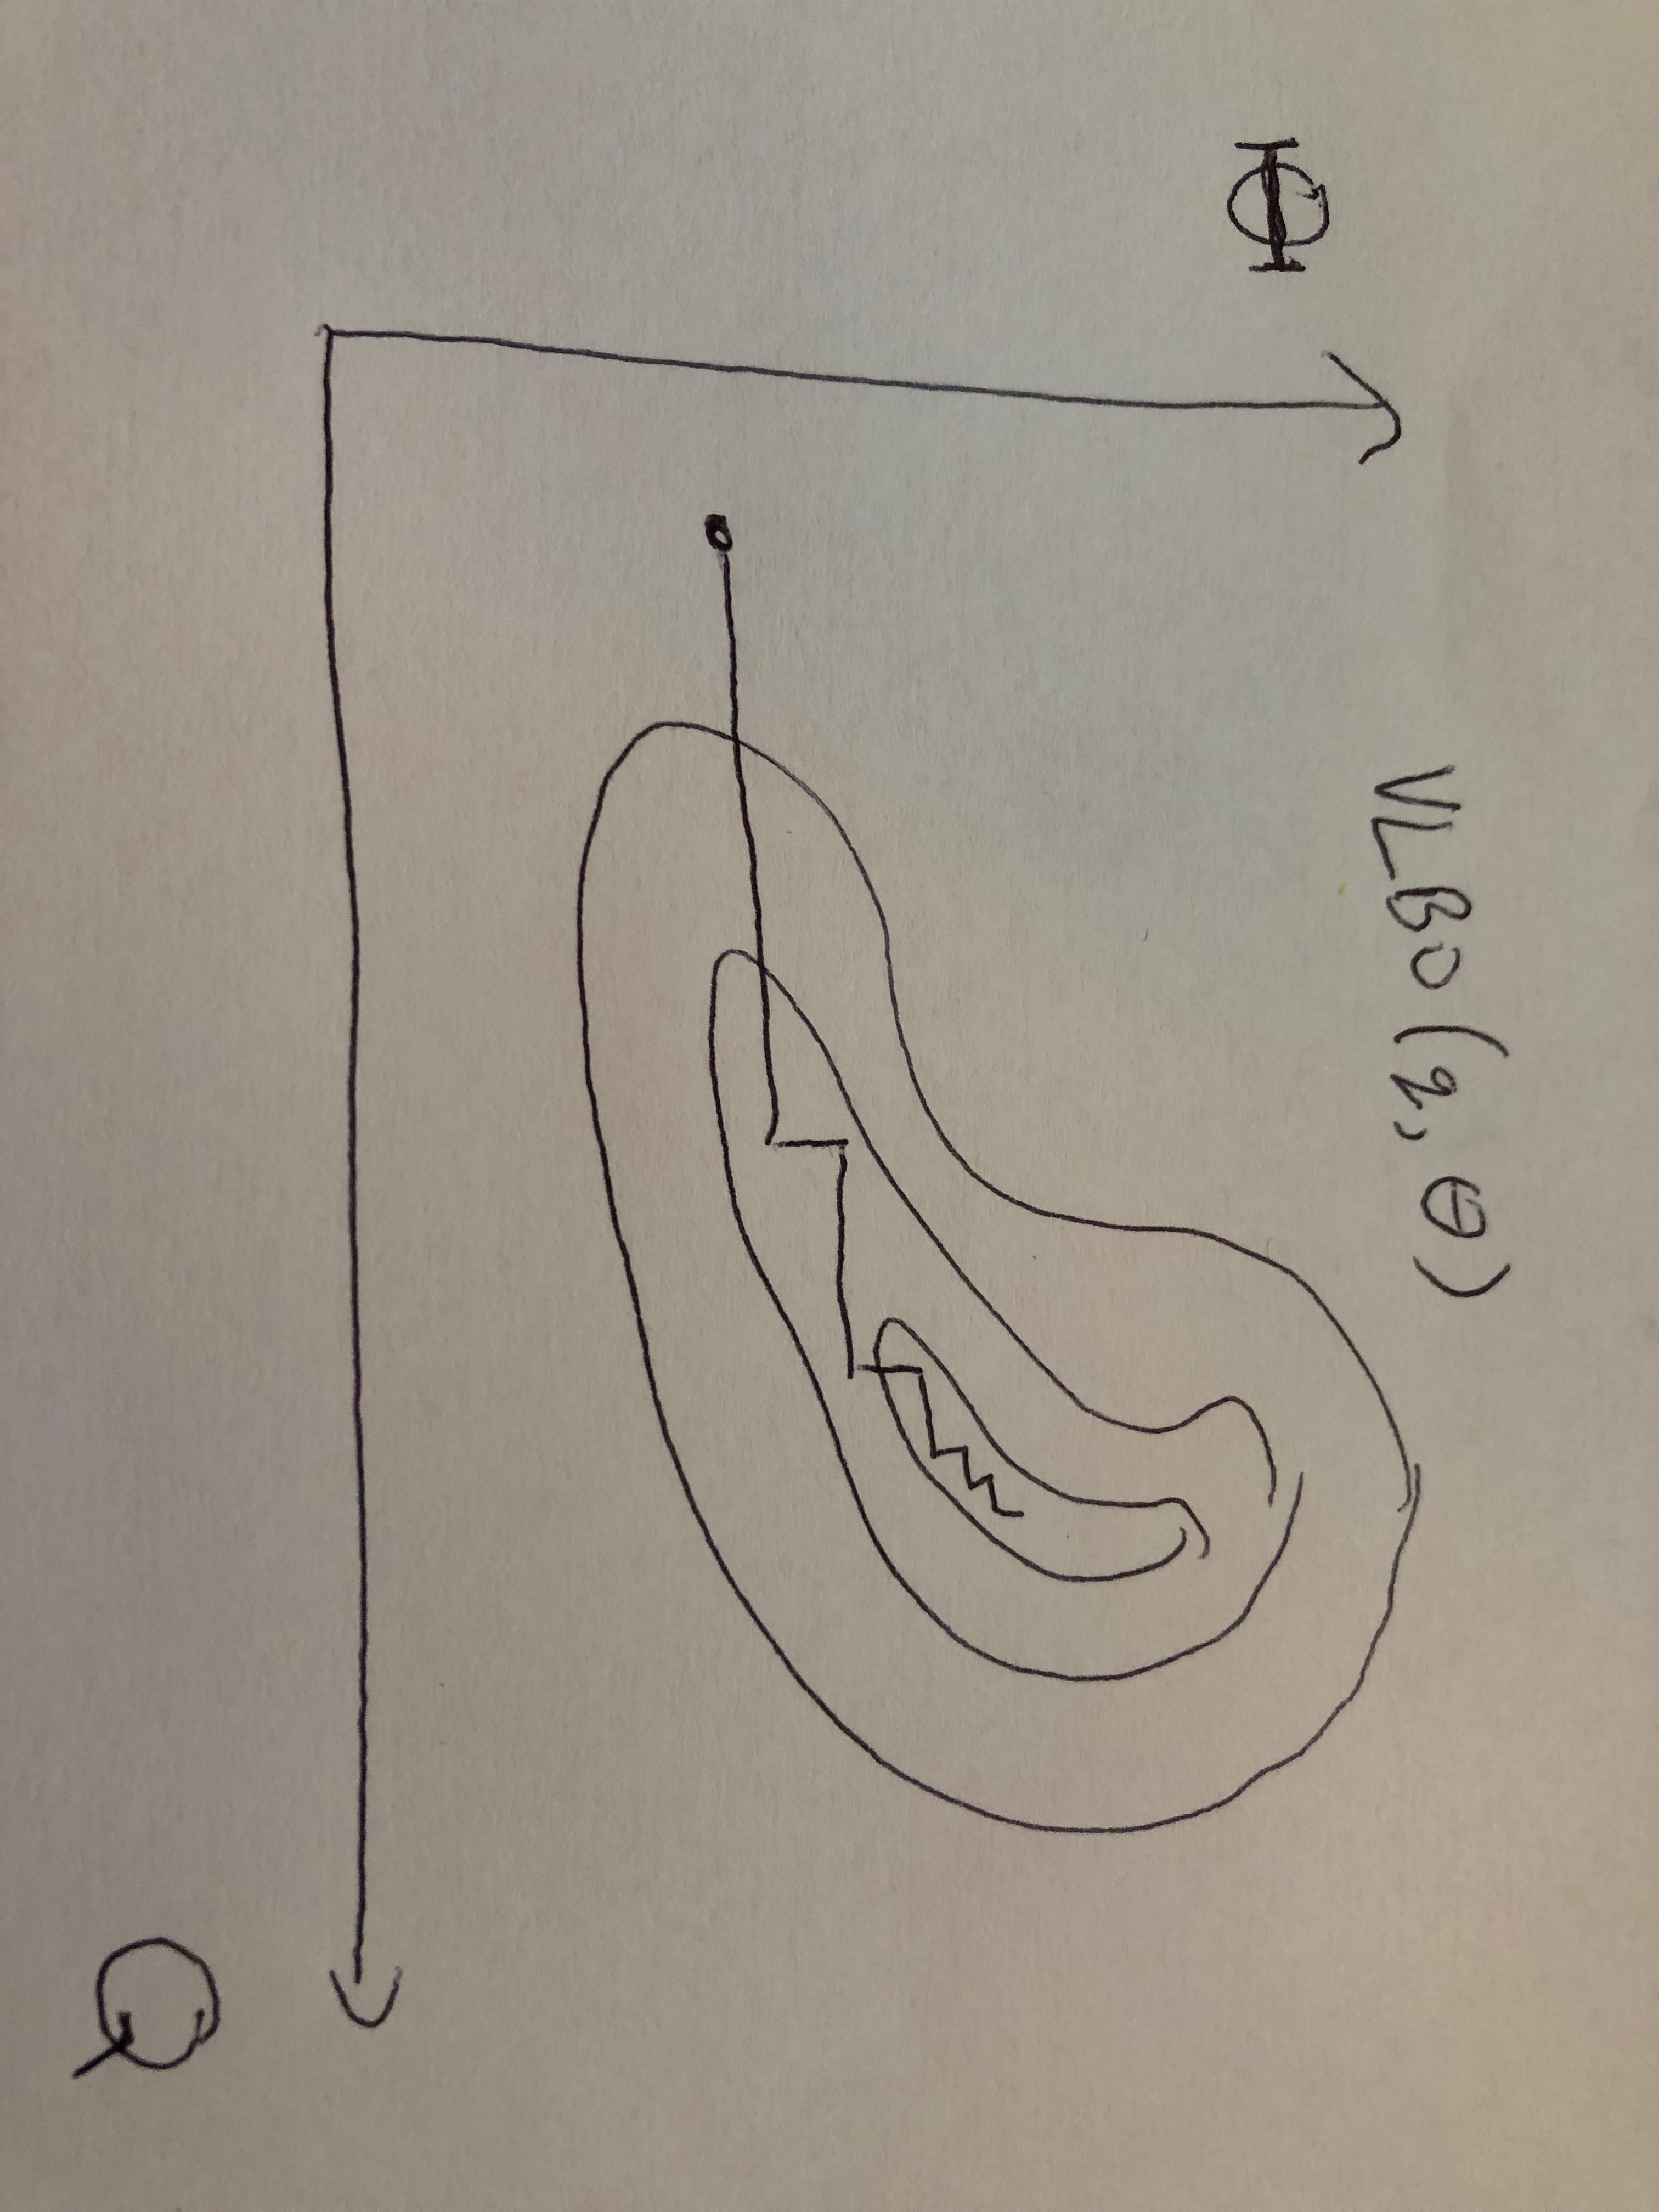
\includegraphics[width=.55\textwidth, angle=90]{images/em_is_perfect_vi.jpg}
	\end{figure}

 
\begin{itemize}
\item If $\Q$ unrestricted, we have EM   
\item What if we restrict $\Q$ ?
%TO SAY: need to for: LDA, BHMM, VAE, BBVI, ADVI,....
\end{itemize}

\end{frame}


\section{The CAVI Algorithm}

\begin{frame}{Mean Field Coordinate Ascent Variational Inference (MF-CAVI)}

\metroset{block=fill}
\begin{block}{Mean field variational families}
A variational family $\Q$ is mean field if it factorizes 

\begin{equation} \label{mean_field}
q(u_1, ..., u_K) = \ds\prod_{k=1}^K q_k(u_k)
\end{equation}
\end{block}

\textit{Mean field coordinate ascent variational inference (MF-CAVI)} iteratively optimizes each variational density, while holding the others fixed. \\
\vfill \vfill 
\pause 
\colorbox{blue!30}{\textbf{Remark.}} Since the $\ELBO$ maps probability densities to a real number, it is a functional, so such optimization can be handled with variational calculus.   
   
\end{frame}

\begin{frame}{Update equations for MF-CAVI}

Given the mean field assumption \eqref{mean_field}, the optimal updates to $\set{q_k}_k$ for coordinate ascent on the $\ELBO$ satisfy 
 
\begin{equation} \label{mfcavi_update}
q_k(u_k) \propto \exp \bigg\{ \E_{q_{-k}} \bigg[  \log p(u_k \cond \+u_{-k}, \+x)\bigg] \bigg\}
\end{equation}
\vfill \vfill 
\pause 
\colorbox{blue!30}{\textbf{Remark.}} The argument to the expectation, known as the \textit{complete conditional}, is what is used in Gibbs sampling.  % So instead of iteratively sampling from the complete conditionals, we take variational expectations with respect to the same distributions.

\vfill \vfill 
\pause 

\colorbox{blue!30}{\textbf{Remark.}} We can also write the update as

\begin{equation} 
q_k(u_k) \propto \exp \bigg\{ \E_{q_{-k}} \bigg[  \log p(\+u, \+x)\bigg] \bigg\}
\label{eqn:mfcavi_update_2}
\end{equation}

which is often referred to as a  \alert{geometric mean}.

%
%%\pause
%
%\alert{Note:} Note that the mean-field assumption \eqref{mean_field} is non-parametric (i.e., no assumptions were made about the parametric family to which $q$ belongs).   The derivation of the update equations  \eqref{mfcavi_update} also has this feature.  Hence, these update equations can be used to determine the optimal parametric families for each of the variational factors.  \\


\end{frame}




\section{Example: Bayesian Gaussian Mixture Model}
\begin{frame}{Example: Bayesian Gaussian Mixture Model}

To see the mean field CAVI algorithm \eqref{eqn:mfcavi_update_2} in a concrete context, consider a version of the Bayesian Gaussian Mixture Model.  
\begin{align*}
\mu_k & \sim \text{Normal}(0, \sigma^2) && k = 1,..., K\\
\+c_i & \sim \text{Categorical}(\pi_1, ..., \pi_K) && i=1, ... ,n \\
x_i \cond \+c_i, \+\mu & \sim \text{Normal}(\+c_i^\top \+\mu, 1) && i = 1,..., n
\end{align*}
\scriptsize (The model is simple in that it assumes that each mixture component has unit variance.) \normalsize 

\pause 
The joint density, by chain rule, is
\[ p(\+x,\+c,\+\mu) = p(\+\mu) \ds\prod_{i=1}^n p(\+c_i) p(x_i \cond \+c_i, \+\mu) \]
\pause 
And a mean-field variational family is given by 
\[  q(\+c, \+\mu) = \ds\prod_{k=1}^K q(\mu_k) \ds\prod_{i=1}^n q(\+c_i) \]

\end{frame}

\begin{frame}{Example: Bayesian Gaussian Mixture Model}
We apply \eqref{eqn:mfcavi_update_2} to determine the coordinate updates for $q_{c_i}$, the variational factors governing cluster assignments.   We take the log of the joint and discard terms that do not depend upon $c_i$ to obtain

\begin{align*}
q(c_{ik}) & \propto \exp \bigg\{ \E_{q_{\mu_k}} \bigg[  \log p(c_i =k) + \log p(x_i \cond c_i=k, \mu) \bigg] \bigg\} \\
& \propto \exp \bigg\{ \E_{q_{\mu_k}} \bigg[ \log \pi_k + x_i \mu_k - \df{1}{2} \mu_k^2 \bigg] \bigg\} \\
& \propto \pi_k \exp \bigg\{ x_i \E_{q_{\mu_k}} [\mu_k] - \df{1}{2}  \E_{q_{\mu_k}} [ \mu_k^2] \bigg\} \\
\end{align*}

The coordinate updates for $q_{\mu_k}$ are derived similarly.  They reveal that $q_{\mu_k}$ are Gaussian, and hence the above expectations are easy to compute. 

\end{frame}

\begin{frame}{Bayesian Gaussian Mixture Model: \\ Updates to mixture component means}
Using the same strategy as when updating cluster assignments $c_i$, we obtain

\begin{align*}
q(\mu_k) & \propto \exp \bigg\{ \E_{-q_{\mu_k}} \bigg[  \log p(\mu_k) + \ds\sum_{i=1}^n \log p(x_i \cond c_i=k, \mu) \bigg] \bigg\} \\
& \propto \exp \bigg\{ -\df{1}{2  \sigma^2} \mu_k^2 +  \ds\sum_{i=1}^{n} \E_{q_c} \bigg[ \+1_{c_i=k}\, \bigg(x_i \mu_k - \df{1}{2} \mu_k^2\bigg) \bigg] \bigg\} \\
& \propto \exp \bigg\{ -\df{1}{2} \bigg(\df{1}{ \sigma^2} + \ds\sum_{i=1}^n q(c_{ik}) \bigg) \mu_k^2 \; +  \;  \bigg( \ds\sum_{i=1}^n q(c_{ik})x_i  \bigg) \mu_k \bigg\} \\
\end{align*}

which is an exponential family distribution with sufficient statistics $(\mu_k, \mu_k^2)$, and hence Gaussian.

\end{frame}




\section{Appendix}

\begin{frame}{MF-CAVI updates on random variables with exponential family complete conditionals} 
Consider a model with unobserved random variables $\+u=(u_1,...,u_k)$.  Let unobserved random variable $u_k$ have a complete conditional in some parametric exponential family $\mathcal{E}$ with natural parameter $\eta_k(u_{-k}, \+x)$.  Let the variational family have mean field factorization $q=q_k(u_k)q_{-k}(u_{-k})$. Then:

\begin{enumerate}
\item The optimal mean field CAVI update \eqref{mfcavi_update} maps the variational factor $q_k$ into $\mathcal{E}$.   \pause 

\item The optimal variational factor $q_k$ has natural parameter $\nu_k$ given by

\begin{align}
\label{eqn:mf_cavi_efcc}
\boxed{\nu_k = \E_{q_{-k}} [\eta_k(u_{-k}, \+x)]}
\end{align}
\pause 
That is, the optimal update sets the natural variational parameter equal to the expectation (with respect to the other variational factors) of the natural parameter of the complete conditional.
\end{enumerate}

\end{frame}


\end{document}

